%!TEX root = ../../Master.tex
\section{Graph theory}

Graph theory is used to model some kind of relationship between objects. These objects could be anything. In graph theory objects are called \enquote{nodes} or \enquote{vertices}. The two terms can be used interchangeably. In this paper, vertices will describe coordinates or POI (points of interest) in a hospital. By definition, each vertex $v$ has a non-empty set of edges $E$. An edge is basically connecting two vertices and thereby providing a relationship between these vertices. Now in order to describe the relationship between two vertices, we use an weighted graph in which an edge has a number attribute called a weight.

We can describe these definitions mathematically.
\begin{align}
	G = (V,E)
	\intertext{where G is a graph, V is a set of vertices and E is a non-empty set of edges}
\end{align}

\begin{figure}[ht!]
    \centering
    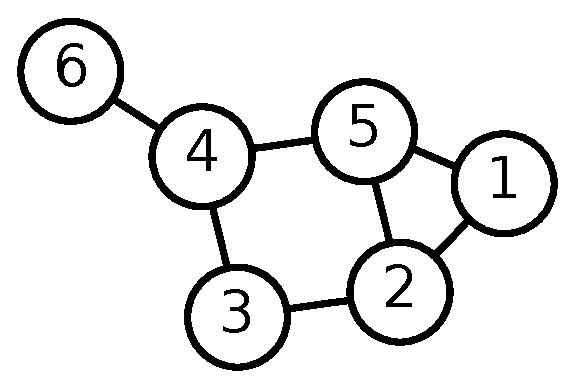
\includegraphics[width=0.5\textwidth]{6n-graf.eps}
    \caption{A labeled simple graph with vertex set $V = \left\{ {1, 2, 3, 4, 5, 6} \right\} $ and edge set $E = \left\{ \left\{ {1,2}\right\}, \left\{ {1,5}\right\}, \left\{ {2,3}\right\}, \left\{ {2,5}\right\}, \left\{ {3,4}\right\}, \left\{ {4,5} \right\} , \left\{ {4,6} \right\} \right\}$. \cite{wiki_graph_glos}}
    \label{fig:graph}
  \end{figure}

\subsection{Storing a complex building as a graph}
\subsubsection{Multiple floors}

A complex such as a hospital usually consist of multiple floors, connected by stairs and elevators as observed at the visit to Sygehus Nord. Representing floors in a graph could be shown by having edges in between different floors. Elevators or stairs represented by vertices that connects the edges between the floors. Having a graph that models the whole complex can have complications such as overlapping vertices coordinates. Estimating a heuristic value between destination and vertices on the other side of, such as floors. Means that the heuristic models that does not account for obstacles, would cause the Astar algorithm to expand vertices, leading to vertices below the destination on a separate floor than the desired.

%indsæt billed her

If the complex is divided into separate floor graphs, the algorithm would not have to account for the z coordinate in its heuristic value. A algorithm could evaluate if the source and destination is on the same floor, if not the algorithm could divide the problem into Astar searches. First finding a path leading to an elevator or stair which lead the destinations floor. The optimal path from one floor to another can be pre-calculated and stored. 

%Indsæt billede her

%Hospitals has many doors and hallways because of their need of rooms for patients, storage and etc.
\subsubsection{Multiple buildings}

The previously described method for modelling floors allows the algorithm to comprehend from complexes of multiple buildings. By only  
A complex can be a collection of multiple building, if  
